% Copyright 2004 by Till Tantau <tantau@users.sourceforge.net>.
%
% In principle, this file can be redistributed and/or modified under
% the terms of the GNU Public License, version 2.
%
% However, this file is supposed to be a template to be modified
% for your own needs. For this reason, if you use this file as a
% template and not specifically distribute it as part of a another
% package/program, I grant the extra permission to freely copy and
% modify this file as you see fit and even to delete this copyright
% notice. 

\documentclass{beamer}

% There are many different themes available for Beamer. A comprehensive
% list with examples is given here:
% http://deic.uab.es/~iblanes/beamer_gallery/index_by_theme.html
% You can uncomment the themes below if you would like to use a different
% one:
%\usetheme{AnnArbor}
%\usetheme{Antibes}
%\usetheme{Bergen}
%\usetheme{Berkeley}
%\usetheme{Berlin}
%\usetheme{Boadilla}
%\usetheme{boxes}
%\usetheme{CambridgeUS}
%\usetheme{Copenhagen}
%\usetheme{Darmstadt}
\usetheme{default}
%\usetheme{Frankfurt}
%\usetheme{Goettingen}
%\usetheme{Hannover}
%\usetheme{Ilmenau}
%\usetheme{JuanLesPins}
%\usetheme{Luebeck}
%\usetheme{Madrid}
%\usetheme{Malmoe}
%\usetheme{Marburg}
%\usetheme{Montpellier}
%\usetheme{PaloAlto}
%\usetheme{Pittsburgh}
%\usetheme{Rochester}
%\usetheme{Singapore}
%\usetheme{Szeged}
%\usetheme{Warsaw}

\usepackage{setspace} 
\usepackage{amsmath}
\usepackage{graphicx}
\newcommand*{\LargerCdot}{\raisebox{-0.25ex}{\scalebox{2.3}{$\cdot$}}}

\usepackage{color}
%\input{rgb}

\definecolor{red1}{rgb}{1.000000,0.000000,0.000000}

\title{Analytics Assignment}

\author{Ranaji~Krishna}

\subject{Theoretical Computer Science}

\pgfdeclareimage[height=0.4cm]{university-logo}{onDeck_logo.jpg}
\logo{\pgfuseimage{university-logo}}

% Let's get started
\begin{document}

\begin{frame}
  \titlepage
\end{frame}

\begin{frame}{Problem Statement}{}
	\begin{itemize}
		\item{Separate $days\_delinquent\_old$ and $days\_delinquent\_new$ into the following groups: $(0, 1-5, 5-10, 10-30, 30-60, 60+)$. Create a transition matrix showing the probability of movement from one group to another. Create another transition matrix showing the probability of movement from one group to another, weighted by outstanding principal balance.} \vspace{0 in} \newline 
	\end{itemize}
\end{frame}

\begin{frame}{Results}{}
	\begin{itemize}		
		\item{Transition Probability Matrix:} \newline			
			\begin{figure}
				\begin{center}
					\vspace*{-0.6 in}
					\hspace*{-0.6in}
					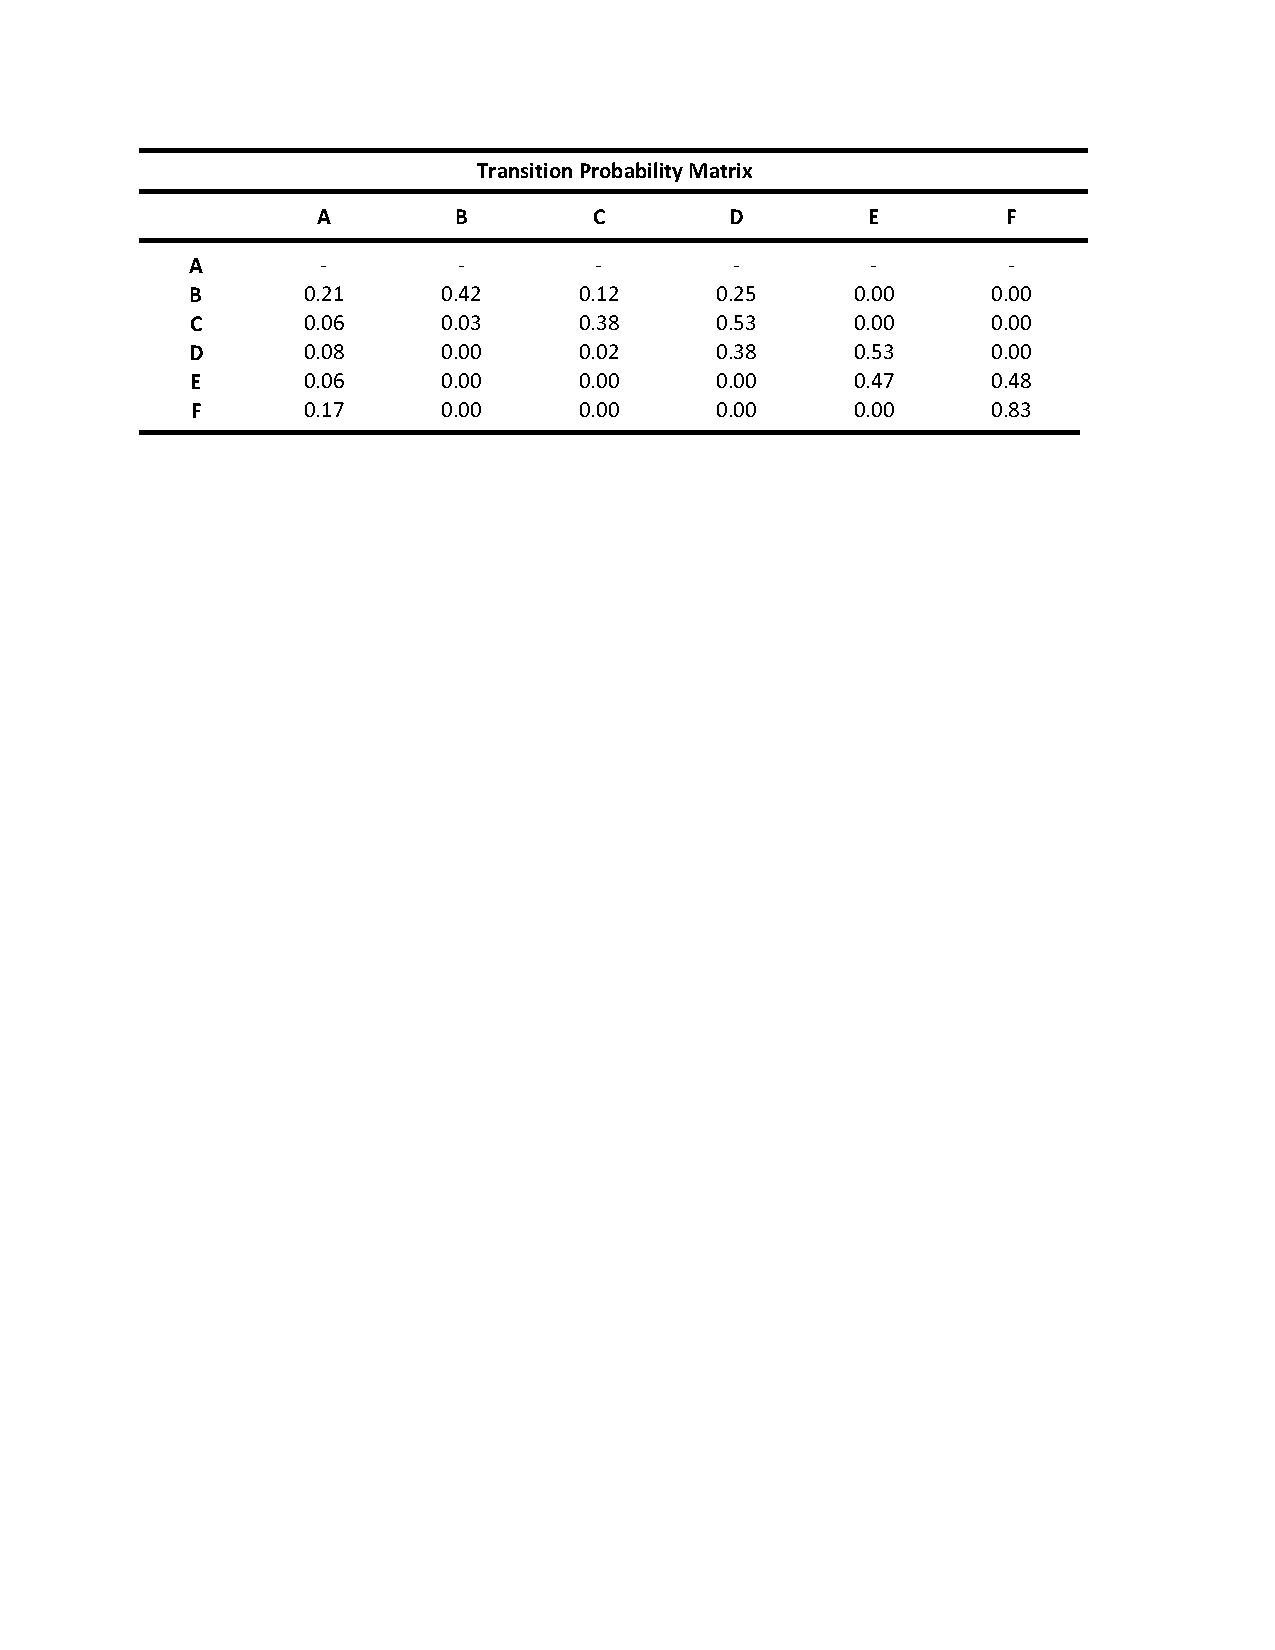
\includegraphics[width=1\textwidth]{trp_mat.pdf} 
				\end{center}
			\end{figure}			
		\vspace{-3.8in}
		\item{Weighted Transition Probability Matrix:} \newline			
			\begin{figure}
				\begin{center}
					\vspace*{-0.6in}
					\hspace*{-0.6in}
					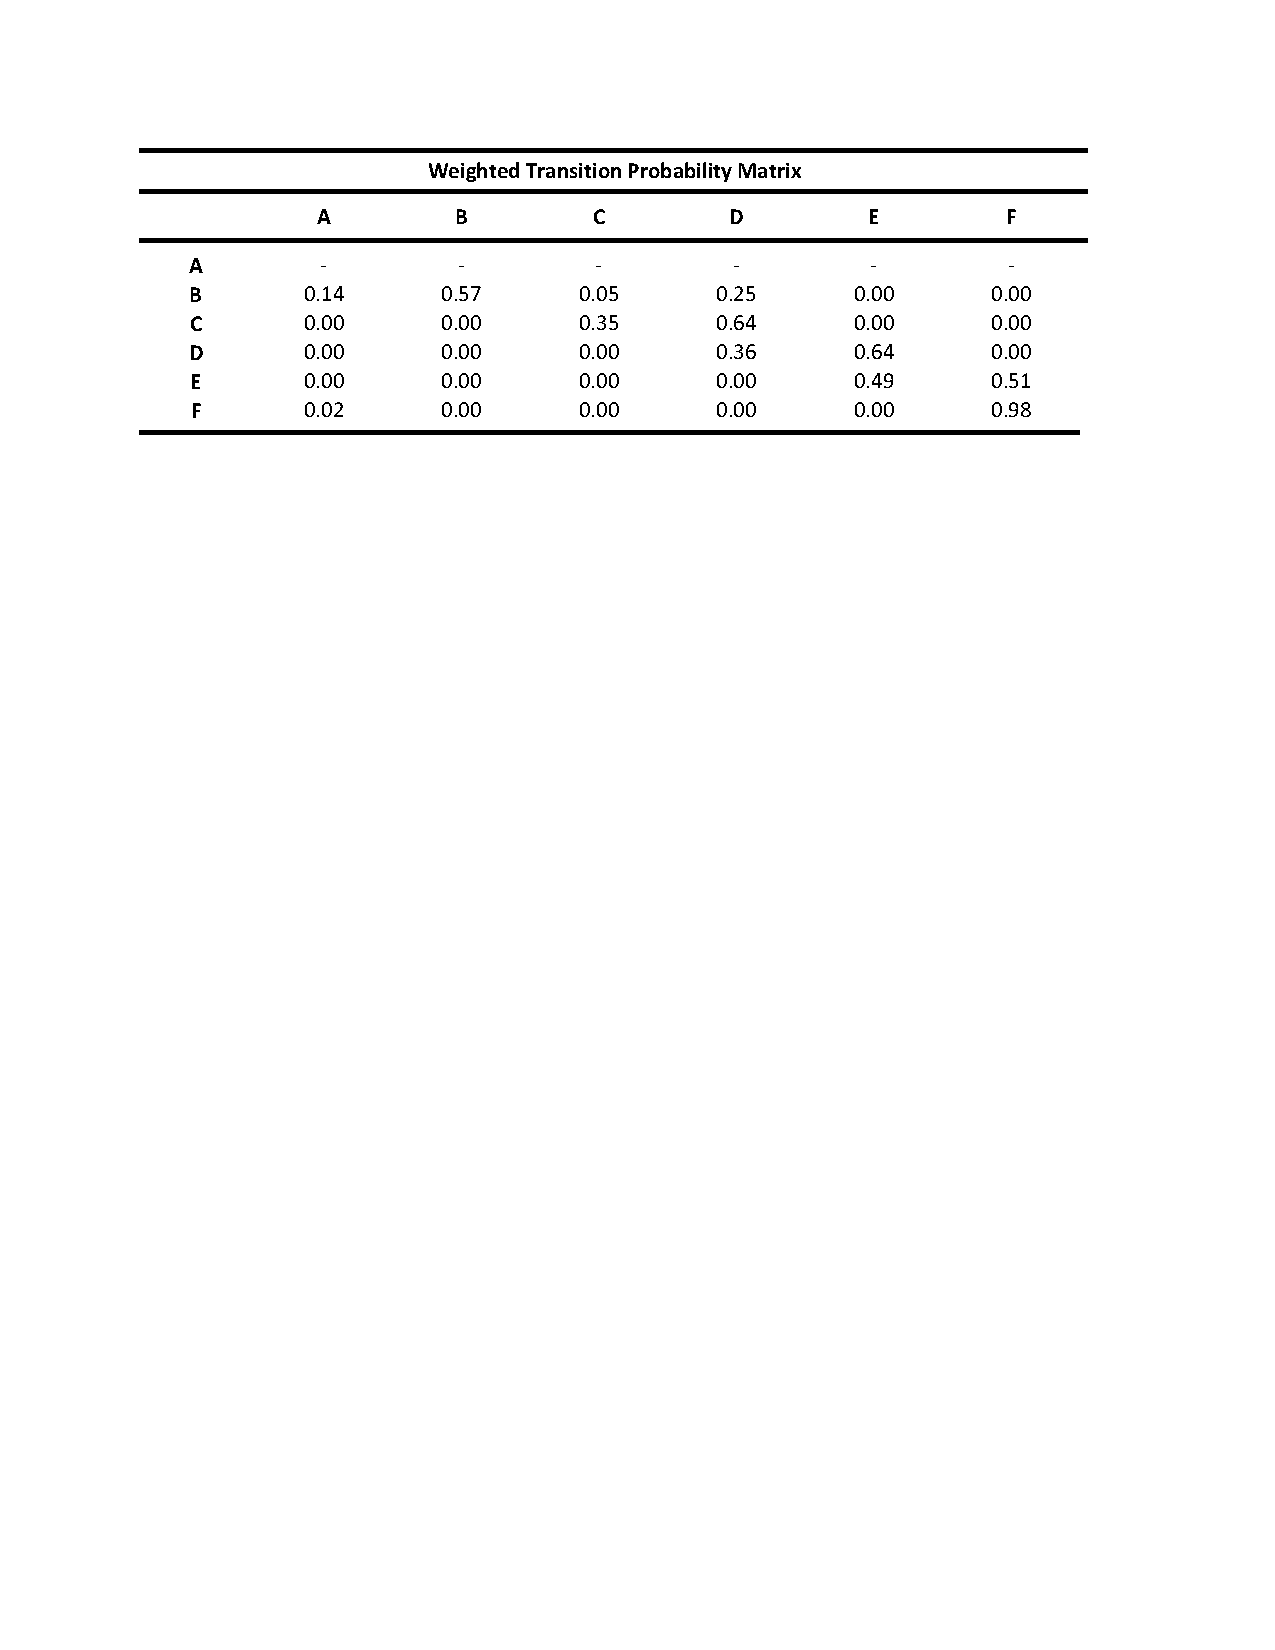
\includegraphics[width=1\textwidth]{wgt_trp_mat.pdf} 
				\end{center}
			\end{figure}
		\vspace{-0.in}
	\end{itemize}
\end{frame}

\begin{frame}{Problem Statement}{}
	\begin{itemize}
		\item{Tell me something interesting about a variable, model, or approach that allows you to distinguish loans whose delinquency is likely to worsen from those whose delinquency is likely to improve.} \vspace{0 in} 
	\end{itemize}
\end{frame}

\begin{frame}{Results}{}
	\begin{itemize}
		\vspace{-0.1 in}		
		\item{We use the {\color{blue}Logistic Regression} model to determine the probability of improvement of a loan delinquency.} \newline\vspace{0 in}
		\item{Loans with improved delinquency are identified by 1 and those with worse delinquency are identified by 0.} \newline\vspace{0 in}
		\item{Loans with no change in delinquency are removed from the data set.} \newline\vspace{0 in}
		\item{The variable $sales\_bin$ quantifies the variable $sales\_channel\_\_c$, where:} \newline\vspace{0 in}
		{\hspace{-0.06in}}{$\LargerCdot$ $1$: ``FAP: Managed Application Program";}\newline 
		{$\LargerCdot$ $2$: ``Referral";}\newline 
		{$\LargerCdot$ $3$: ``Direct";}\newline
		{$\LargerCdot$ delinquency of loans under ``Promonotory" did not change.}
		\vspace{-0.in}
	\end{itemize}
\end{frame}

\begin{frame}{Results}{contd.}
	\vspace{-0.25in}
	\begin{itemize}
		\item{Summary of Logistic Regression:} \newline
		\begin{figure}
		\vspace{-0.1 in}
			\begin{center}
					\vspace*{-0.3 in}
					\hspace*{-0.2in}
					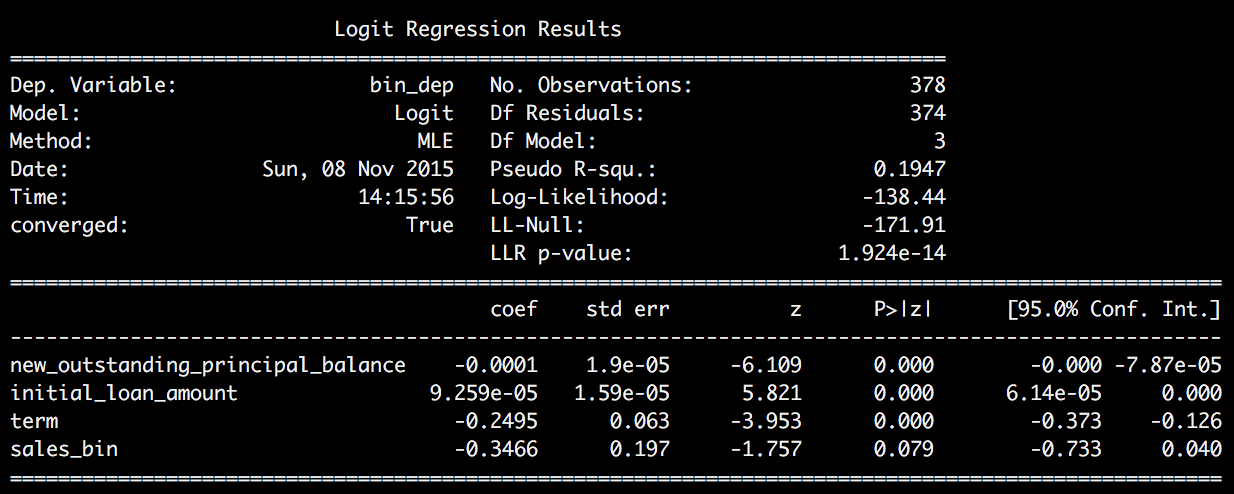
\includegraphics[width=1\textwidth]{log_reg_results.png} 
				\end{center}
		\end{figure}
		\item{Significant coefficients as odds ratio:} \newline\vspace{-0 in}		
		\begin{figure}
			\begin{center}
				\vspace*{-0.2in}
				\hspace*{-2in}
				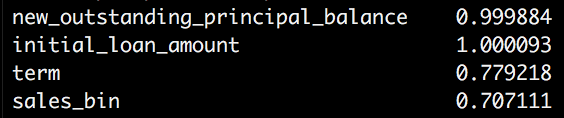
\includegraphics[width=0.55\textwidth]{odds_ratio.png} 
				\end{center}
		\end{figure}
	\end{itemize}
\end{frame}

\begin{frame}{Results}{contd.}
	\begin{figure}
	\vspace{-0.15 in}
		\begin{itemize}\item{Perfromance of the estimator} \newline\vspace{-0 in}
			\begin{center}
				\vspace*{-0.21 in}
				\hspace*{-1in}
				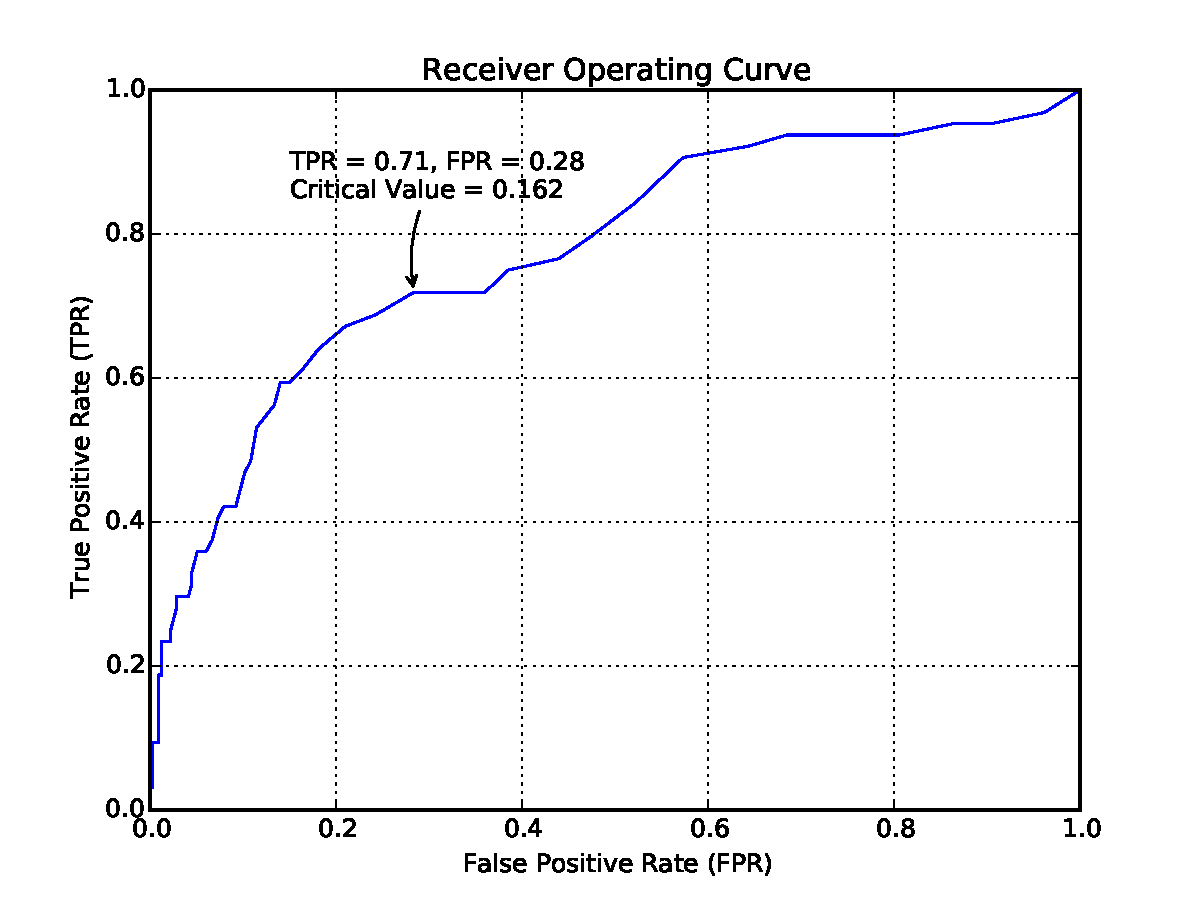
\includegraphics[width=0.9\textwidth]{ROC.pdf} 
			\end{center}
		\end{itemize}
	\end{figure}
		\vspace{-0.in}
\end{frame}

\begin{frame}{Insights}{}
	\begin{itemize}		
		\item{The delinquency of a loan for which the model generates a probability of improvement of greater than $0.16$ (the critical-value) has a $71\%$ chance of improvement. However, there is a $28\%$ chance of the delinquency worsening.} \newline\vspace{0 in}
		\item{The $Term$ and the $Sales\_Channel$ of a loan have a major influence on the odds of improvement:} \newline\vspace{0 in}
		{\hspace{-0.06in}}{$\LargerCdot$ an increase in $Term$ of $1$ month reduces the odds of improvement by $22\%$;}\newline
		{$\LargerCdot$ the odds of improvement decreases by $29\%$ if the $Sales\_Channel$ is a ``Referral" compared to an ``FAP: Managed Application Program". The odds decrease by $29\%$ if the $Sales\_Channel$ is  ``Direct" compared to if it is a ``Referral".}
		\end{itemize}
\end{frame}


\begin{frame}{}{}
	\begin{center}
        		\Large{END}          
      \end{center}
\end{frame}

\end{document}
